\documentclass[a4j,fleqn,10pt]{jsarticle}
\usepackage{ipsj}
\usepackage{txfonts}
\usepackage[symbol*,perpage]{footmisc}
\usepackage[dvipdfm]{graphicx, color}

%-------------------------------------------jtitle and jauthors information
\begin{document}

\jtitle{誤りパターン埋込み型ステガノグラフィに関する一考察}
\jcontact{松江工業高等専門学校\dag}
\jauthor{索手 一平\dag}

\maketitle


%-------------------------------------------document
\section{はじめに}
本研究はテキスト情報をグレースケール画像に埋め込むようなステガノグラフィ
技術を対象とする。


\section{ステガノグラフィ}
ステガノグラフィとはある情報を他のデータに埋め込む技術・研究分野の総称
であり、これによって情報が埋め込まれていること自体を隠すことができるため
主に秘密情報の伝達において利用されている。ステガノグラフィ技術ではその特
徴からなるべく多くの情報を埋め込めること、そして情報が隠蔽されていること
を主観的・客観的に認知されないことが重要となる。

\section{LSB法}
LSB法とはステガノグラフィ技術の最も代表的な埋め込み方式の一つである。こ
の手法はカバーデータのLSB平面をテキスト情報のバイナリ表現とそのまま置き
換えることによって、情報の埋め込みを行う。アルゴリズムが単純であり実装が
容易であるがその一方で埋め込み時のビット誤りについての考慮がなされておら
ず、画像の劣化を招きやすいという欠点がある。

\section{誤りパターン埋め込み法}
誤りパターン埋め込み法とはLSB法を元に考案された手法である。この手法では
テキスト情報をより冗長でハミング重みの小さなビット列である誤りパターンに
変換し、誤りパターンと画像のLSB平面との排他的論理和でLSB平面を置き換える
ことによって、情報の埋め込みを行う。LSB法に比べ誤りビットが少なくなるた
め画質の劣化を招きにくくなるが、より冗長なビット列に変換することから埋め
込める情報量が少なくなるという欠点がある。

\section{誤りパターンへの変換方法}
誤りパターンへの変換方法の一つに埋め込みデータと誤りパターンを対応付けた
テーブルを用意する方法が知られている。しかし、この方法の問題点として埋め
込みデータの大きさに比例してテーブルが膨大となりメモリ制約の大きい環境で
の実装が困難になるという点があげられる\cite{Paper01}。そこで本研究ではShalkwijkの数え
上げ符号\cite{Paper02}を用いた埋め込みデータから誤りパターンを動的に背制する手法を提案
する。

\section{複数の画像を用いての画質劣化の検証実験}
実験手順の概要を図1に示す。実験手順は以下のとおりである。また、埋め込み
に使用するメッセージはほぼ当確率で発生する8bitコードの列とする。
\begin{enumerate}
\renewcommand{\labelenumi}{(\arabic{enumi})}
 \item メッセージの各コードをShalkwijkの数え上げ符号を用いて誤りパターン
       に変換し、画像のLSB平面との履いた低論理和をLSB平面に埋め込む。
 \item 埋め込み前後の画像を比較し、誤り率、PSNR値、SSIMを算出する。
 \item 誤りパターン長を増加させながら(1)、(2)を繰り返す。
 \item 画像を入れ替えて(3)を繰り返す。
\end{enumerate}

\begin{figure}[htbp]
 \begin{center}
  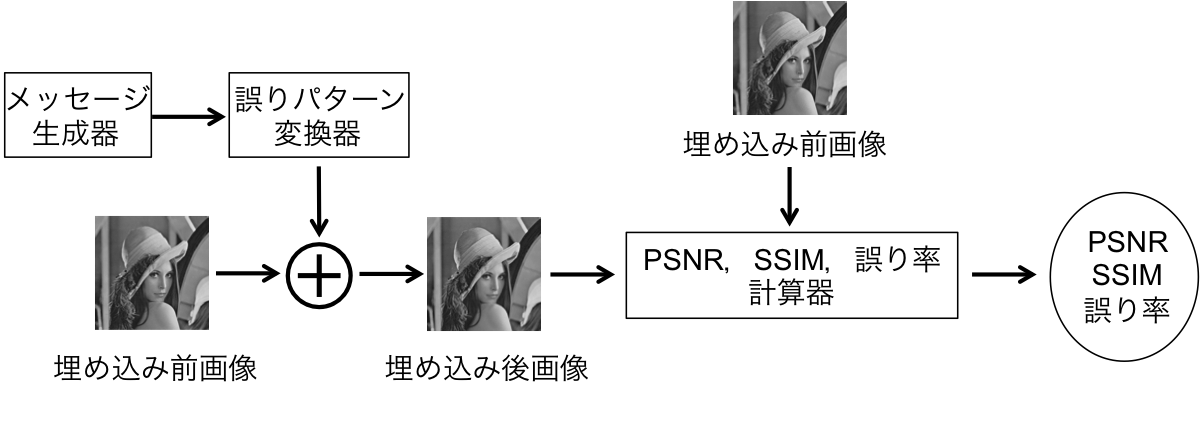
\includegraphics[width=8cm]{experiment1.png}
 \end{center}
 \caption{実験概要2}
\end{figure}

\section{実験結果}
PSNRと誤り率、SSIMと誤り率のトレードオフについてのグラフをそれぞれ図1,
2に、各画像事のSSIMの変化についてのグラフを図3に示す。今回の実験では
web上で収集した256☓256pxの8bitグレイスケールBitmapである自然画像を20枚使
用し実験を行った。

\section{考察}
図3より画像ごとに画質劣化の傾向に差異があることがわかったため、それらの
画像を並べ主観的に観察を行ったところ、近しい画素値を持つピクセルの大きい
塊、つまりコントラストの小さい部分が大きい画像ほど画質劣化が大きくなる傾向がわかった。これを客観的に評価す
るために次の実験を行った。

\section{実験}
実験手順の概要を図5に示す。実験手順は以下のとおりである。

\begin{enumerate}
\renewcommand{\labelenumi}{(\arabic{enumi})}
 \item 画素値を30の区間にわけ、各区間内の画素値とそれ以外の画素値で2値化
       を行い、それらに対し4近傍でのラベリング処理を行い、最も大きい面積
       部分を算出する。
 \item (1)をすべての画像に対し繰り返す。
 \item 5で算出したSSIMとのピアソンの相関係数を算出する。
\end{enumerate}

\begin{figure}[htbp]
 \begin{center}
  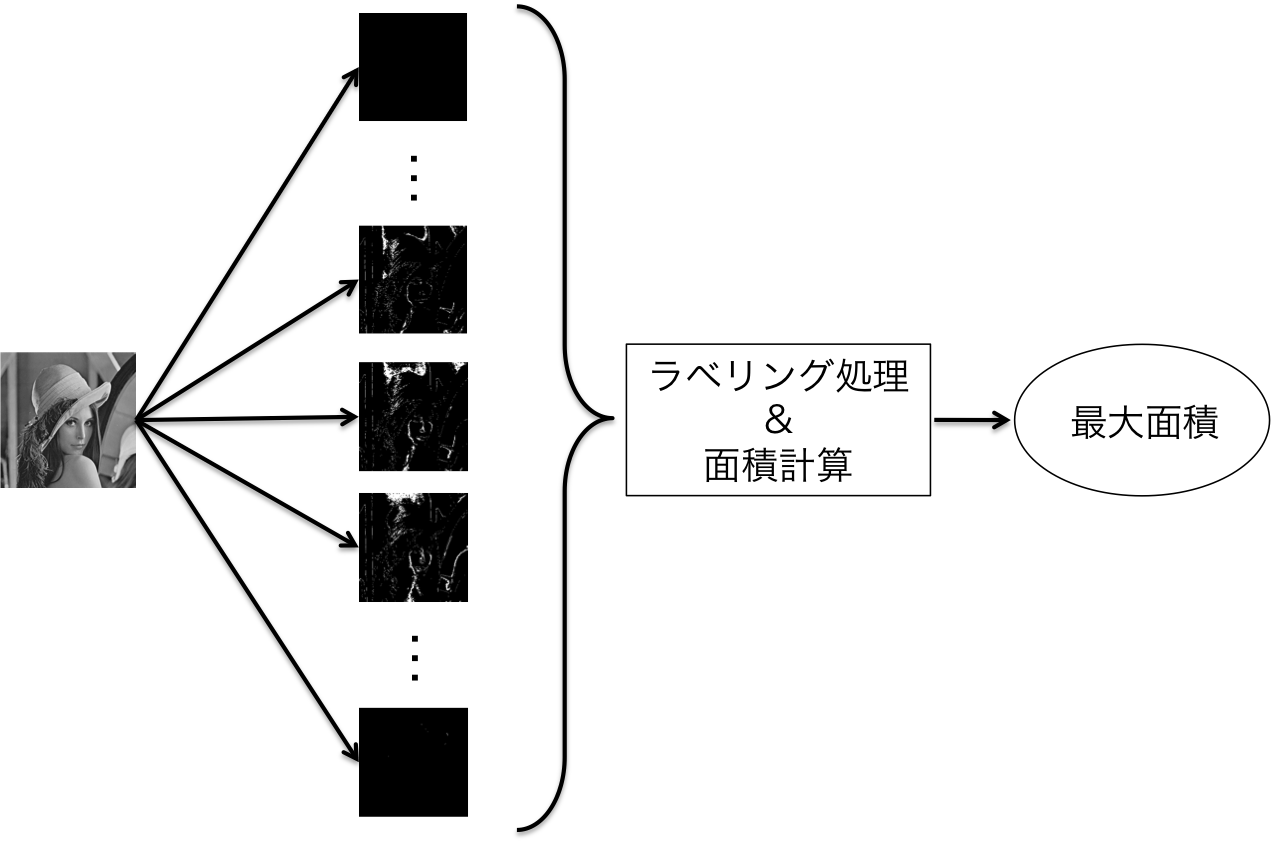
\includegraphics[width=8cm]{experiment2.png}
 \end{center}
 \caption{実験概要2}
\end{figure}

\section{実験結果}
上記の実験を行った結果、約0.6という相関が得られた。

\section{考察}
これまでの実験から近しい画素値の大きい集合をもつ画像ほど画質の視覚的な画
質劣化が大きくなるという結果が得られた。これは画素間のコントラストが大き
いほどメッセージ埋め込み後の画素値変化が目立ちにくいため得られたのだと考
えられる。

%-------------------------------------------etitle and eauthors information
\footnotetext[0]{\hspace*{-5.2mm}A study on steganography based on embedding error patterns}
\footnotetext[1]{\hspace*{-6.5mm}\dag Ippei Nawate}
\footnotetext[2]{\hspace*{-6.5mm}\dag Matsue College Of Technology}

%-------------------------------------------references
\bibliographystyle{junsrt}
\bibliography{draft}

\end{document}
